\documentclass[11pt,a4paper]{article}
\usepackage[spanish,es-nodecimaldot]{babel}	% Utilizar español
\usepackage[utf8]{inputenc}					% Caracteres UTF-8
\usepackage{graphicx}						% Imagenes
\usepackage[hidelinks]{hyperref}			% Poner enlaces sin marcarlos en rojo
\usepackage{fancyhdr}						% Modificar encabezados y pies de pagina
\usepackage{float}							% Insertar figuras
\usepackage[textwidth=390pt]{geometry}		% Anchura de la pagina
\usepackage[nottoc]{tocbibind}				% Referencias (no incluir num pagina indice en Indice)
\usepackage{enumitem}						% Permitir enumerate con distintos simbolos
\usepackage[T1]{fontenc}					% Usar textsc en sections
\usepackage{amsmath}						% Símbolos matemáticos

\usepackage{listings}
\usepackage[dvipsnames]{xcolor}

\definecolor{codegreen}{rgb}{0,0.6,0}
\definecolor{codegray}{rgb}{0.5,0.5,0.5}
\definecolor{codepurple}{rgb}{0.58,0,0.82}
\definecolor{backcolour}{rgb}{0.95,0.95,0.92}

\lstdefinestyle{mystyle}{
    backgroundcolor=\color{backcolour},   
    commentstyle=\color{codegreen},
    keywordstyle=\color{magenta},
    numberstyle=\tiny\color{codegray},
    stringstyle=\color{codepurple},
    basicstyle=\ttfamily\footnotesize,
    breakatwhitespace=false,         
    breaklines=true,                 
    captionpos=b,                    
    keepspaces=true,                 
    numbers=left,                    
    numbersep=5pt,                  
    showspaces=false,                
    showstringspaces=false,
    showtabs=false,                  
    tabsize=4,
    language=C++
}

\usepackage{fancyvrb}

% redefine \VerbatimInput
\RecustomVerbatimCommand{\VerbatimInput}{VerbatimInput}%
{fontsize=\footnotesize,
 %
 commandchars=\|\(\), % escape character and argument delimiters for
                      % commands within the verbatim
 commentchar=*        % comment character
}

\lstset{style=mystyle}

% Comando para poner el nombre de la asignatura
\newcommand{\asignatura}{Arquitectura y Computación de Altas Prestaciones}
\newcommand{\autor}{Vladislav Nikolov Vasilev}
\newcommand{\titulo}{Práctica 4}
\newcommand{\subtitulo}{Suma de vectores con CUDA}
\newcommand{\rama}{Ingeniería de Computadores}

% Comando vector
\renewcommand{\vec}[1]{\mathbf{#1}}

% Configuracion de encabezados y pies de pagina
\pagestyle{fancy}
\lhead{\autor{}}
\rhead{\asignatura{}}
\lfoot{Grado en Ingeniería Informática}
\cfoot{}
\rfoot{\thepage}
\renewcommand{\headrulewidth}{0.4pt}		% Linea cabeza de pagina
\renewcommand{\footrulewidth}{0.4pt}		% Linea pie de pagina

\begin{document}
\pagenumbering{gobble}

% Pagina de titulo
\begin{titlepage}

\begin{minipage}{\textwidth}

\centering

%
\includegraphics[scale=0.5]{img/ugr.png}\\

\includegraphics[scale=0.3]{img/logo_ugr.jpg}\\[1cm]

\textsc{\Large \asignatura{}\\[0.2cm]}
\textsc{GRADO EN INGENIERÍA INFORMÁTICA}\\[1cm]

\noindent\rule[-1ex]{\textwidth}{1pt}\\[1.5ex]
\textsc{{\Huge \titulo\\[0.5ex]}}
\textsc{{\Large \subtitulo\\}}
\noindent\rule[-1ex]{\textwidth}{2pt}\\[3.5ex]

\end{minipage}

%\vspace{0.5cm}
\vspace{0.7cm}

\begin{minipage}{\textwidth}

\centering

\textbf{Autor}\\ {\autor{}}\\[2.5ex]
\textbf{Rama}\\ {\rama}\\[2.5ex]
\vspace{0.3cm}


\includegraphics[scale=0.3]{img/etsiit.jpeg}

\vspace{0.7cm}
\textsc{Escuela Técnica Superior de Ingenierías Informática y de Telecomunicación}\\
\vspace{1cm}
\textsc{Curso 2019-2020}
\end{minipage}
\end{titlepage}

\pagenumbering{arabic}
\tableofcontents
\thispagestyle{empty}				% No usar estilo en la pagina de indice

\newpage

\setlength{\parskip}{1em}

\section{Introducción}

En esta práctica se pide implementar dos versiones de un mismo programa: una primera
versión secuencial y una versión en \texttt{CUDA}. El objetivo del programa es, dados
dos vectores $\vec{A}$ y $\vec{B}$, ambos de tamaño $n$, obtener un vector de salida
$\vec{C}$ del mismo tamaño en el que $\forall \vec{C}_i \in \vec{C}$, su valor
venga determinado por la expresión:

\begin{equation}
\vec{C}_i =
\Bigg(
\bigg(
\frac{\log(5 \cdot \vec{A}_i \cdot 100 \cdot \vec{B}_i) + 7 \cdot \vec{A}_i}{0.33}
\bigg)^3 \Bigg)^7
\label{eq:formula}
\end{equation}

Además, se ha especificado que los vectores de entrada $\vec{A}$ y $\vec{B}$
se tienen que replicar un número de veces, de forma que su longitud se vea incrementada.
En este caso, se ha decidido \textbf{que se van a tener 5 copias de los vectores originales},
es decir, que los vectores van a tener una longitud de $5n$, donde $n$ es el tamaño
original especificado en los archivos proporcionados.

De los diez problemas proporcionados se han descartado los problemas 3 y 9 debido a que
tienen los mismos tamaños que otros problemas, más en concreto tienen los mismos tamaños que los
problemas 0 y 4, respectivamente. Para cada uno de los ocho problemas restantes se van a tomar
medidas de tiempo de lo que se tarda en hacer todas las operaciones con los dos programas.
Con ellas se representará la evolución del tiempo de ejecución en cada caso en función
del tamaño del problema y se hará un estudio de la ganancia.

Adicionalmente, se pide que se obtengan las especificaciones de la \texttt{GPU} que se está
utilizando, de manera que se tenga más infomración sobre esta.

\section{Especificaciones de la \texttt{GPU}}

Primeramente vamos a ver cuáles son las especificaciones de la \texttt{GPU} que vamos a
utilizar. Para ello se ha creado un programa que puede encontrarse en el archivo
\texttt{deviceProperties.cu}, el cuál muestra la siguiente información:

\begin{itemize}
  \item Nombre del dispositivo.
  \item Número de SMs (procesadores).
  \item Número de SPs por SM (cores por procesador).
  \item Número total de SPs.
  \item Memoria total de la gráfica en MB.
  \item Memoria compartida por SM en KB.
  \item Memoria compartida por bloque en KB.
  \item Número máximo de hebras por bloque.
  \item Número máximo de hebras por cada dimensión.
\end{itemize}

El código que muestra esta información es el siguiente:

\begin{lstlisting}
int n_devices;

cudaGetDeviceCount(&n_devices);

int i;

for (i = 0; i < n_devices; i++)
{
	cudaDeviceProp prop;
	cudaGetDeviceProperties(&prop, i);
	int numSPs = getSPcores(prop);

	printf("Device number: %d\n", i);
	printf(" Device name: %s\n", prop.name);
	printf(" Number of SMs: %d\n", prop.multiProcessorCount);
	printf(" Number of SPs per SM: %d\n", numSPs);
	printf(" Total Number of SPs: %d\n",
			numSPs * prop.multiProcessorCount);
	printf(" Total Available Global Memory Size (MB): %zu\n",
			prop.totalGlobalMem / (1<<20));
	printf(" Shared Memory Per SM (KB): %zu\n",
			prop.sharedMemPerMultiprocessor / (1<<10));
	printf(" Shared Memory Per Block (KB): %zu\n",
			prop.sharedMemPerBlock / (1<<10));
	printf(" Max. Threads Per Block: %d\n", prop.maxThreadsPerBlock);
	printf(" Max. Threads Per Dimension: x: %d, y: %d, z: %d\n",
			prop.maxThreadsDim[0], prop.maxThreadsDim[1], prop.maxThreadsDim[2]);
}
\end{lstlisting}

La función \texttt{getSPcores} se ha extraído de una respuesta a una pregunta en
\textit{StackOverflow} \cite{cuda-sp}. En caso de tener más de una tarjeta gráfica
(que no es el caso), se mostraría la información para cada una de ellas. En este
caso se ha obtenido la siguiente información:

\VerbatimInput{../out/specs.txt}

\section{Versión secuencial}

Una vez que hemos visto las especificaciones de nuestra gráfica, vamos a ver cómo sería
una primera versión secuencial del programa.

La versión secuencial carga los ficheros de datos que se han especificado como parámetros,
carga los valores, los copia un número de veces que se determina como parámetro y realiza
la operación, obteniendo el vector $\vec{C}$ de salida. La función que realiza el cálculo
que se puede ver en la ecuación \eqref{eq:formula} es la siguiente:

\begin{lstlisting}
void add_vectors(float *A, float *B, float *C, int N)
{
    int i;

    for (i = 0; i < N; i++)
    {
        C[i] = pow(pow(log(5*A[i]*100*B[i] + 7*A[i]) / 0.33, 3), 7);
    }
}
\end{lstlisting}

La función recibe como parámetro los dos vectores de entrada, el de salida y el
tamaño de los vectores, y con un bucle recorre los elementos de $\vec{A}$ y $\vec{B}$
y calcula el correspondiente elemento de $\vec{C}$.

El resto del código se encuentra en el archivo \texttt{vectorAdd.c} y se puede consultar
de ser necesario. Como en general son operaciones sencillas, no se van a explicar ni a incluir
aquí, ya que no se considera que estén relacionadas con la asignatura (lectura de ficheros,
reserva de memoria, etc.).

\section{Versión paralela con \texttt{CUDA}}

Una vez implementada y probada la versión secuencial se ha procedido a desarrollar
la versión paralela. El código de esta versión puede encontrarse en el archivo
\texttt{vectorAdd.cu}, pero vamos a comentar aquí algunas de las partes
más importantes.

Lo primero es la función que aplica la operación de la ecuación \eqref{eq:formula}
sobre los elementos de los vectores $\vec{A}$ y $\vec{B}$. En este caso se
ha declarado dicha función como un \textit{kernel} de \texttt{CUDA}, y su implementación
puede verse a continuación:

\begin{lstlisting}
__global__ void addVectorsKernel(float *d_A, float *d_B, float *d_C, int N)
{
    int i = blockIdx.x * blockDim.x + threadIdx.x;

    if (i < N)
    {
        d_C[i] = pow(pow(log(5*d_A[i]*100*d_B[i] + 7*d_A[i]) / 0.33, 3), 7);
    }
}
\end{lstlisting}

Cuando se especifica el \textit{kernel}, \texttt{\_\_global\_\_} significa que
el \textit{kernel} se llama desde el anfitrión o \textit{host} y se ejecuta
en el dispositivo o \textit{device} (es decir, en la tarjeta gráfica). La posición del
elemento $i$-ésimo que se va a calcular viene determinada por el índice del bloque,
el tamaño del bloque y el índice de la hebra dentro del bloque. Una vez que se
ha determinado la posición es necesario comprobar que dicho valor no excede el
tamaño de los vectores (podría darse en el caso en el que en un bloque haya más
hebras que elementos restantes del vector, por ejemplo).

Dentro del programa principal también han habido algunos cambios. En el siguiente fragmento
de código se puede ver lo más destacable de las modificaciones llevadas a cabo:

\begin{lstlisting}
// Allocate CUDA arrays
float *d_A, *d_B, *d_C;

cudaMalloc(&d_A, N * sizeof(float));
cudaMalloc(&d_B, N * sizeof(float));
cudaMalloc(&d_C, N * sizeof(float));

// Set number of threads and blocks
int DIM_BLOCK = 128;
int DIM_GRID = ((N - 1) / DIM_BLOCK) + 1;
    
// Add vectors and retrieve information from device
t1 = omp_get_wtime();
    
// Copy values
cudaMemcpy(d_A, h_A, N * sizeof(float), cudaMemcpyHostToDevice);
cudaMemcpy(d_B, h_B, N * sizeof(float), cudaMemcpyHostToDevice);

addVectorsKernel<<<DIM_GRID, DIM_BLOCK>>>(d_A, d_B, d_C, N);

cudaMemcpy(h_C, d_C, N * sizeof(float), cudaMemcpyDeviceToHost);

t_time = omp_get_wtime() - t1;
\end{lstlisting}

Vemos que lo primero que se hace es declarar los arrays que van a estar en el dispositivo
y se reserva memoria para ellos. Una vez reservada la memoria se procede a
determinar el tamaño del bloque (\texttt{DIM\_BLOCK}) y el número de bloques o tamaño del
\textit{grid} (\texttt{DIM\_GRID}). Se ha especificado que el tamaño del bloque sea de 128
hebras debido a que es un múltiplo de 32, que es el tamaño del \textit{warp} de hebras que
es planificado y enviado a ejecutar, además de que es el mismo número que el de SPs por SM,
lo cuál permitiría ejecutar un bloque entero a la vez en un SM. Aparte, se han hecho algunas
pruebas con distintos tamaños de bloque y este ha dado unos resultados bastante buenos, con lo
cuál se considera que, en general, puede funcionar bien para distintos tamaños. Por otra parte,
el número de bloques se ha escogido según la siguiente expresión:

\begin{equation}
\texttt{DIM\_GRID} = \frac{N - 1}{\texttt{DIM\_BLOCK}} + 1
\label{eq:dim-grid}
\end{equation}

\noindent donde $N$ es el número de elementos del vector y la fracción es una división
entera. Al escoger el número de bloques de esta forma nos aseguramos de que siempre sea
el número exacto de bloques, aunque en uno de ellos no se usen todas las hebras para hacer
cómputos. Si calculásemos el número de bloques como $\frac{N}{\texttt{DIM\_BLOCK}}$ el resultado
solo sería correcto si $N$ fuese múltiplo del tamaño del bloque. En el caso de que por ejemplo
$N$ fuese menor a dicho tamaño, el resultado sería 0, lo cuál no debería ser posible,
ya que siempre tiene que haber al menos un bloque. Si $N$ no fuese un múltiplo entonces al
hacer la división se estaría subestimando el número de bloques necesarios, ya que el resultado
de la división entera sería menor al número real de bloques necearios.

Habiendo hecho esto llega la sección en la que se miden los tiempos, donde se ejecuta el
\textit{kernel} declarado anteriormente. Primero se copian los vectores \texttt{h\_A}
y \texttt{h\_B} en las correspondientes variables. Es importante destacar que a la hora
de copiar se especifica el parámetro \texttt{cudaMemcpyHostToDevice}, el cuál indica que
se copie del \textit{host} al dispositivo (la tarjeta gráfica). Una vez hecho esto
se ejecuta el \textit{kernel} de la forma que se puede ver en la línea 22.
Finalmente se copian los datos del vector que está en el dispositivo al vector que se encuentra
en el \textit{host} (línea 24) y se mide la diferencia de tiempos. Es importante destacar que en
esta ocasión para transferir los datos del dispositivo al \textit{host} se ha especificado la
opción \texttt{cudaMemcpyDeviceToHost}.

\section{Experimentación y resultados}

Una vez que hemos visto cómo se han implementado las dos versiones vamos a hacer la
experimentación. Tal y como se ha dicho anteriormente, se van a tener 5 copias de los dos
vectores de entrada, de forma que el tamaño original se verá multiplicado por 5. A la hora
de compilar los programas no se ha utilizado optimización, de forma que la comparación sea
justa.

Se han medido los tiempos para cada problema probado y se han ordenado dichas medidas
según el tamaño del problema (el tamaño de los vectores de entrada). Se han creado tanto una
tabla como una gráfica que muestran los resultados. Una vez hecho esto, se ha calculado la
ganancia para un tamaño determinado con la siguiente expresión:

\begin{equation}
S_{tam} = \frac{T^{tam}_s}{T^{tam}_p}
\end{equation}

Una vez dicho esto, vamos a ver los resultados obtenidos para la versión secuencial y la
paralela de forma conjunta. A continuación se puede ver la tabla de tiempos, acompañada
de su correspondiente gráfica:

\begin{table}[H]
\centering
\begin{tabular}{|c|c|c|}
\hline
\textbf{\begin{tabular}[c]{@{}c@{}}Tamaño de\\ los vectores\end{tabular}} & \textbf{\begin{tabular}[c]{@{}c@{}}Tiempo secuencial\\ (s)\end{tabular}} & \textbf{\begin{tabular}[c]{@{}c@{}}Tiempo CUDA\\ (s)\end{tabular}} \\ \hline
500 & 0.000357 & 0.000049 \\ \hline
5125 & 0.000952 & 0.000086 \\ \hline
10240 & 0.001887 & 0.000139 \\ \hline
20480 & 0.003761 & 0.00025 \\ \hline
25000 & 0.004338 & 0.000298 \\ \hline
30000 & 0.005056 & 0.000361 \\ \hline
45000 & 0.007283 & 0.000512 \\ \hline
163840 & 0.02738 & 0.001758 \\ \hline
\end{tabular}
\caption{Tiempo de ejecución secuencial y paralelo con \texttt{CUDA} para cada problema.}
\label{tab:times}
\end{table}

\begin{figure}[H]
  \centering
  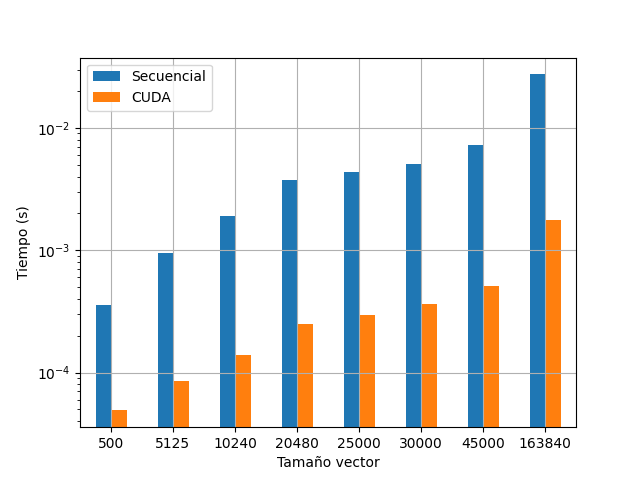
\includegraphics[scale=0.6]{img/seq-cuda}
  \caption{Evolución del tiempo de ejecución del programa secuencial y el programa en
  \texttt{CUDA} en función del tamaño del vector con escala logarítmica en el eje $Y$.}
  \label{fig:seq-cuda}
\end{figure}

Vemos, como es obvio, que los tiempos de la versión secuencial son mucho mayores que los
de la versión paralela en \texttt{CUDA}. Esto se debe a que las instrucciones del procesador
de la CPU están optimizadas para que tarden muy pocos ciclos, mientras que las de la
tarjeta no lo están, pero al ser procesadores de tipo SIMT
(\textit{Single Instruction Multiple Threads}), pueden ejecutar una misma
instrucción sobre múltiples hebras a la vez, lo cuál permite reducir drásticamente los tiempos
de ejecución al procesar una mayor cantidad de información a la vez.

Vemos también que en ambos casos los tiempos de ejecución van aumentando de manera parecida
a medida que va aumentando el tamaño del problema, lo cuál es esperable. El ratio al que crecen
es más o menos parecido excepto al principio, es decir, cuando se pasa de 500 a 20480 elementos.
En este caso, el tiempo secuencial experimenta un crecimiento algo más pronunciado que el
paralelo, pero a partir de ahí parece que crecen en más o menos la misma medida, estando,
obviamente, siempre el tiempo paralelo varios órdenes de magnitud por debajo del secuencial.

Al observar los tiempos podemos sacar también una serie de conclusiones. Una de ellas es que, al
estar el tiempo de ejecución en la \texttt{GPU} por debajo del secuencial para todos los tamaños,
podemos afirmar que en todos los casos ha merecido la pena paralelizar, ya que siempre
hemos tardado menos tiempo con el programa paralelo. Para problemas más grandes, las diferencias
de tiempo también serán bastante notables, ganando siempre la \texttt{GPU}.

Por la forma en la que crecen los tiempos podemos concluir también que, para problemas más
pequeños que el más pequeño que aparece reflejado en la gráfica, el tiempo de ejecución del
programa secuencial podría ser menor al del paralelo, debido a que no habría transferencia de
datos entre la memoria principal y la memoria global del dispositivo, lo cuál es un gran cuello
de botella y donde se pasa una gran cantidad de tiempo. Por tanto, eso nos indicaría que
para problemas realmente pequeños utiliar la tarjeta gráfica sería como matar moscas
a cañonazos.

Finalmente, el hecho de que el tiempo de ejecución del programa paralelo vaya creciendo nos
indica que hay muchos bloques que están a la espera de que el planificador los seleccione.
Esto se debe a que disponemos de una gráfica con unos pocos SM, los cuáles están ocupados
la mayoría del tiempo, y por tanto, la mayoría de bloques estarán a la espera durante
bastante tiempo. Si tuviésemos más SMs, quizás los tiempos podrían ser algo menores.

Una vez que hemos analizado los tiempos, vamos a hacer un pequeño estudio de la ganancia.
A continuación se ofrece una tabla con los valores obtenidos según el tamaño del problema
de forma ordenada (como en el caso anterior), además de una gráfica que muestra la evolución
de la ganancia:

\begin{table}[H]
\centering
\begin{tabular}{|c|c|}
\hline
\textbf{\begin{tabular}[c]{@{}c@{}}Tamaño de\\ los vectores\end{tabular}} & \textbf{Ganancia} \\ \hline
500 & 7.28571429 \\ \hline
5125 & 11.06976744 \\ \hline
10240 & 13.57553957 \\ \hline
20480 & 15.044 \\ \hline
25000 & 14.55704698 \\ \hline
30000 & 14.00554017 \\ \hline
45000 & 14.22460938 \\ \hline
163840 & 15.5745165 \\ \hline
\end{tabular}
\caption{Ganancia para cada problema.}
\label{tab:speedup}
\end{table}

\begin{figure}[H]
  \centering
  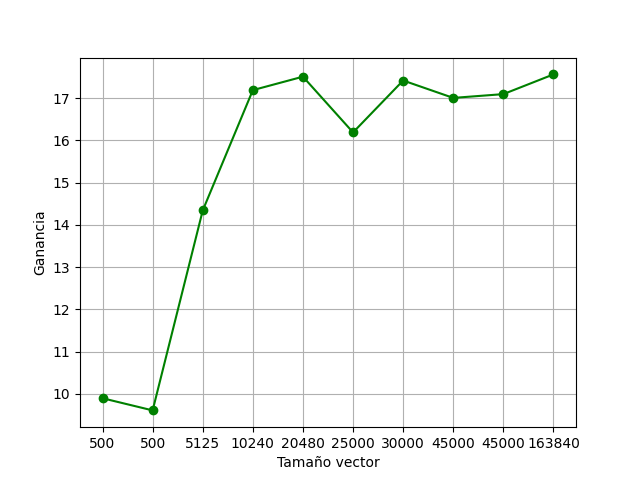
\includegraphics[scale=0.6]{img/speedup}
  \caption{Ganancia obtenida en función del tamaño del vector.}
\end{figure}

Tal y como podemos ver en la gráfica y en la tabla, la ganancia obtenida es bastante grande y
va aumentando a medida que aumenta el tamaño de los vectores de entrada. Empieza con un
valor algo más grande que 7 y va creciendo hasta llegar a un valor próximo a 15, y a partir
de ahí va subiendo y bajando pero manteniéndose próxima a este valor. El motivo por el
que se producen bajadas se debe a que en algunos casos la tasa de crecimiento del tiempo
secuencial es algo inferior a la del tiempo paralelo, haciendo por tanto que la ganancia
sea menor.

Podemos ver que la ganancia crece mucho entre los 500 y los 20480 elementos. Esto se
debe a que, tal y como comentamos anteriormente, los tiempos secuenciales crecen mucho
más rápido que los paralelos en estos casos. A partir de ahí, la ganancia oscial alrededor
de 15, bajando en algunos casos por los motivos comentados anteriormente, y subiendo de
nuevo hacia el final. Posiblemente, si probásemos con un problema mucho más grande, la ganancia
obtenida podría estar en torno a 15 o aproximarse ligeramente a 16 debido a que los tiempos
secuencial y paralelo crecen de forma más o menos pareja para problemas grandes.

Parece que, en general, la ganancia máxima que se puede conseguir con esta tarjeta es
de aproximadamente 15, tal y como hemos comentado. Si tuviésemos una tarjeta gráfica más
potente y con más SMs, los tiempos posiblemente serían mucho más pequeños, lo cuál a su vez
supondría una mayor ganancia. No obstante, tener una ganancia cercana a 15 para problemas grandes
no es ninguna tontería. Por ejemplo, un problema muy grande que tardase unos 60 minutos en la
versión secuencial podría ser resuelto por la versión paralela en tan solo 4 minutos, lo cuál
nos muestra la abismal diferencia que hay entre la versión paralela y la secuencial.
Por tanto, a pesar de que la \texttt{GPU} no sea todo lo potente que quisiéramos, nos permite
resolver resolver problemas grandes en mucho menos tiempo, y por tanto, merece la pena
paralelizarlos mediante \texttt{CUDA}.

\section{Conclusiones}

El uso de \texttt{GPUs} ha permitido acelerar muchísimo los cómputos de grandes cantidades
de datos. Esto es gracias a que utilizan procesadores de tipo SIMT, los cuáles permiten
ejecutar las mismas instrucciones sobre un gran número de hebras a la vez en vez de ejecutar las
instrucciones una detrás de otra de forma secuencial (en el caso de programas secuenciales,
que es con lo que hemos estado comparando el rendimiento de nuestra tarjeta gráfica).

Las \texttt{GPUs} permiten obtener una ganancia extremadamente alta y son muy útiles en
programas que manejen grandes cantidades de datos, como cálculo muy intensivo, gráficos,
\textit{machine learning} y, sobre todo, en \textit{deep learning}, donde juegan un papel
fundamental en el entrenamiento de las redes profundas.

No obstante, es de menester recordar que las tarjetas gráficas no son la solución a todos
los problemas. Por ejemplo, si estamos ante un problema que requiera mucha sincronización
y/o comunicación, posiblemente lo mejor sería escoger otro paradigma/lenguaje, ya que
las tarjetas gráficas están especializadas sobre todo en problemas del tipo SPMD, mientras que
para otro tipo de problemas como por ejemplo maestro/esclavo no son tan buenas. Además, los
tiempos de comunicación entre el \textit{host} y el dispositivo pueden llegar a ser bastante
elevados, con lo cuál si no se dispone de una cantidad de datos suficiente, la mayor parte del
tiempo se va a estar enviando y recibiendo la información, lo cuál negaría completamente
cualquier ganancia que permita obtener la tarjeta si una versión secuencial es capaz de
hacerlo en el mismo tiempo. Otra cosa que hay que tener en cuenta es que, debido a que todas
las hebras ejecutan el mismo código, introducir bloques condicionales en los \textit{kernels}
es contraproducente, ya que solo se relantizaría el tiempo de ejecución, haciendo que la
ejecución sea casi secuencial.

Por tanto, debemos, antes de nada, entender el tipo de problema al que nos estamos enfrentando,
determinar cuál es la mejor metodología a seguir y resolverlo con las herramientas más adecuadas.


\newpage

\begin{thebibliography}{5}

\bibitem{cuda-sp}
StackOverflow. \textit{How can I get number of Cores in cuda device?}
\\\url{https://stackoverflow.com/questions/32530604/how-can-i-get-number-of-cores-in-cuda-device}

\end{thebibliography}

\end{document}

